\documentclass[reprint,english,notitlepage]{revtex4-1}  % defines the basic parameters of the document

% if you want a single-column, remove reprint

% allows special characters (including æøå)
\usepackage[utf8]{inputenc}
\usepackage[english]{babel}

%% note that you may need to download some of these packages manually, it depends on your setup.
%% I recommend downloading TeXMaker, because it includes a large library of the most common packages.

\usepackage{physics,amssymb}  % mathematical symbols (physics imports amsmath)
\usepackage{graphicx}         % include graphics such as plots
\usepackage{xcolor}           % set colors
\usepackage{hyperref}         % automagic cross-referencing (this is GODLIKE)
\usepackage{tikz}             % draw figures manually
\usepackage{listings}         % display code
\usepackage{subfigure}        % imports a lot of cool and useful figure commands
\usepackage{cprotect}
\usepackage{float}

% defines the color of hyperref objects
% Blending two colors:  blue!80!black  =  80% blue and 20% black
\hypersetup{ % this is just my personal choice, feel free to change things
    colorlinks,
    linkcolor={red!50!black},
    citecolor={blue!50!black},
    urlcolor={blue!80!black}}

%% Defines the style of the programming listing
%% This is actually my personal template, go ahead and change stuff if you want
\lstnewenvironment{python}{
	\lstset{ %
		inputpath=,
		backgroundcolor=\color{white!88!black},
		basicstyle={\ttfamily\scriptsize},
		commentstyle=\color{magenta},
		language=Python,
		morekeywords={True,False},
		tabsize=4,
		stringstyle=\color{green!55!black},
		frame=single,
		keywordstyle=\color{blue},
		showstringspaces=false,
		columns=fullflexible,
		keepspaces=true}
}{}

\lstnewenvironment{cpp}{
	\lstset{ %
		inputpath=,
		backgroundcolor=\color{white!88!black},
		basicstyle={\ttfamily\scriptsize},
		commentstyle=\color{magenta},
		language=C++,
		morekeywords={True,False},
		tabsize=4,
		stringstyle=\color{green!55!black},
		frame=single,
		keywordstyle=\color{blue},
		showstringspaces=false,
		columns=fullflexible,
		keepspaces=true}
}{}

\lstset{literate=
  {á}{{\'a}}1 {é}{{\'e}}1 {í}{{\'i}}1 {ó}{{\'o}}1 {ú}{{\'u}}1
  {Á}{{\'A}}1 {É}{{\'E}}1 {Í}{{\'I}}1 {Ó}{{\'O}}1 {Ú}{{\'U}}1
  {à}{{\`a}}1 {è}{{\`e}}1 {ì}{{\`i}}1 {ò}{{\`o}}1 {ù}{{\`u}}1
  {À}{{\`A}}1 {È}{{\'E}}1 {Ì}{{\`I}}1 {Ò}{{\`O}}1 {Ù}{{\`U}}1
  {ä}{{\"a}}1 {ë}{{\"e}}1 {ï}{{\"i}}1 {ö}{{\"o}}1 {ü}{{\"u}}1
  {Ä}{{\"A}}1 {Ë}{{\"E}}1 {Ï}{{\"I}}1 {Ö}{{\"O}}1 {Ü}{{\"U}}1
  {â}{{\^a}}1 {ê}{{\^e}}1 {î}{{\^i}}1 {ô}{{\^o}}1 {û}{{\^u}}1
  {Â}{{\^A}}1 {Ê}{{\^E}}1 {Î}{{\^I}}1 {Ô}{{\^O}}1 {Û}{{\^U}}1
  {œ}{{\oe}}1 {Œ}{{\OE}}1 {æ}{{\ae}}1 {Æ}{{\AE}}1 {ß}{{\ss}}1
  {ű}{{\H{u}}}1 {Ű}{{\H{U}}}1 {ő}{{\H{o}}}1 {Ő}{{\H{O}}}1
  {ç}{{\c c}}1 {Ç}{{\c C}}1 {ø}{{\o}}1 {å}{{\r a}}1 {Å}{{\r A}}1
  {€}{{\euro}}1 {£}{{\pounds}}1 {«}{{\guillemotleft}}1
  {»}{{\guillemotright}}1 {ñ}{{\~n}}1 {Ñ}{{\~N}}1 {¿}{{?`}}1
}



\usepackage{thmtools}
\DeclareMathOperator{\nullspace}{Nul}
\DeclareMathOperator{\collspace}{Col}
\DeclareMathOperator{\rref}{Rref}
%%\DeclareMathOperator{\dim}{Dim}

 % "meq": must be equal
\newcommand{\meq}{\overset{!}{=}}

\newcommand{\R}{\mathbb{R}}
\newcommand*\Heq{\ensuremath{\overset{\kern2pt L'H}{=}}}
\usepackage{bm}
\newcommand{\uveci}{{\bm{\hat{\textnormal{\bfseries\i}}}}}
\newcommand{\uvecj}{{\bm{\hat{\textnormal{\bfseries\j}}}}}
\DeclareRobustCommand{\uvec}[1]{{%
  \ifcsname uvec#1\endcsname
     \csname uvec#1\endcsname
   \else
    \bm{\hat{\mathbf{#1}}}%
   \fi
}}
\usepackage[binary-units=true]{siunitx}

\makeatletter
\newcommand*{\balancecolsandclearpage}{%
  \close@column@grid
  \cleardoublepage
  \twocolumngrid
}
\makeatother

\newcounter{subproject}
\renewcommand{\thesubproject}{\alph{subproject}}
\newenvironment{subproj}{
\begin{description}
	\item[\refstepcounter{subproject}(\thesubproject)]
}{\end{description}}


\begin{document}
\title{On the implementation and usage of Jacobi's rotational algorithm to solve the buckling beam problem, as well as the ground-state energies of a one-electron and two-electron quantum dot system.}   % self-explanatory
\author{Eivind Støland, Anders P. Åsbø}               % self-explanatory
\date{\today}                             % self-explanatory
\noaffiliation                            % ignore this

\begin{abstract}
Many problems can be rewritten as eigenvalue problems, which means that being able to solve eigenvalue problems numerically is important. In this report we present an implementation of Jacobi's rotation algorithm and use it to solve three different physical problems of varying complexity. We solve the problem of a buckling beam and a quantum harmonic oscillator with both one and two electrons. All these problems reduce to a wave equation which can be represented as an eigenvalue problem by approximating a second order derivative.

The numerical solution to the buckling beam problem seems to be in agreement with the analytical results. However, there is a larger error in both quantum harmonic oscillator problems, with the two-electron problem having the largest error. As there are significant sources of errors not related to the algorithm applied to solve these, these results tell little about the error caused by the algorithm itself. Further research would be necessary in order to use these problems to further evaluate our implementation of the algorithm, and the amount of research seemingly necessary would warrant a study of its own.

We performed a benchmark of our implementation, and compared it to the built-in eig\_sym solver from the Armadillo C++ library. The benchmark revealed our Jacobi solver to be faster for the matrix used in the buckling beam problem, but slower for the matrix used in the two-electron problem. We concluded that our jacobi solver works well for simple symmetric matrices, but eig\_sym is better suited for more complicated symmetric matrices.
\end{abstract}


\maketitle                                % creates the title, author, date


\tableofcontents

\section{Introduction} \label{sec:I}

Some of the most important physical problems can be formulated numerically as eigenvalue problems. Thus being able to find eigenvalues and eigenvectors numerically is of critical importance. There are several methods and algorithms that can be used for this, and in this report we study Jacobi's rotation algorithm, and discuss its merits and failings. We also apply it on three different problems, namely that of a buckling beam, and that of one and two electrons in a quantum harmonic oscillator potential. In general this algorithm is applicable to any physical problem which can be formulated as an eigenvalue problem with a symmetrical matrix.

These three problems showcase some key differences, however. The buckling beam problem results in a Toeplitz matrix, which makes it easier to use this problem to test how well the algorithm works. The single electron in a quantum harmonic oscillator potential results in the diagonal elements of the matrix no longer being constant, and the problem with two electrons result in yet more complex diagonal elements because of the Coulomb interaction between the electrons. This creates some specific error sources that we discuss in detail in \hyperref[sec:III:b]{section III.B.}

Precision of the solutions is key, and thus we test the accuracy of the result against analytical answers for all three problems. For the buckling beam we compare the first numerical eigenvector against the analytical one, and in the two quantum harmonic oscillator problems we compare numerical and analytical eigenvalues. We also make an estimate on how many FLOPs at most which will be needed in order for the solution to converge. This lets us evaluate the computational cost of the algorithm.

\section{Formalism} \label{sec:II}

\subsection{Unitary transformations and eigenvalues} \label{sec:II:a}

We define a unitary transformation of a matrix \textbf{A} into a matrix \textbf{B} as:

\begin{align*}
\textbf{B} = \textbf{U}^T \textbf{AU} \, ,
\end{align*}

where \textbf{U} is a unitary matrix ($\textbf{U}^T\textbf{U} = \textbf{I}$, where \textbf{I} is the identity matrix). This type of transformation will preserve the eigenvalues of the system, meaning that \textbf{A} and \textbf{B} share the same eigenvalues. This can be seen by manipulating the eigenvalue equation for \textbf{A}:

\begin{align*}
\textbf{A}\textbf{v} = \lambda \textbf{v} \, ,
\end{align*}

where $\lambda$ is the eigenvalue belonging to eigenvector \textbf{v}. We multiply by $\textbf{U}^T$ from the left and add the identity matrix in between \textbf{A} and \textbf{x}, and use that $\textbf{U}^T \textbf{U} = \textbf{UU}^T$:

\begin{align*}
\textbf{U}^T \textbf{AIv} &= \lambda \textbf{U}^T \textbf{v} \\
\textbf{U}^T \textbf{AU}^T \textbf{Uv} &= \lambda \textbf{U}^T \textbf{v} \\
(\textbf{U}^T \textbf{AU} ) (\textbf{U}^T \textbf{v}) &= \lambda (\textbf{U}^T \textbf{v}) \\
\textbf{Bw} &= \lambda \textbf{w} \, ,
\end{align*}

where we have defined $\textbf{w} = \textbf{U}^T \textbf{v}$. This is now an eigenvalue equation for \textbf{B} with $\lambda$ as the eigenvalue belonging to eigenvector \textbf{w}. This shows that the eigenvalues of the matrix is preserved through a unitary transformation.

A unitary transformation of an orthogonal set of vectors $\textbf{v}_i$ will conserve the orthogonality of the set of vectors. We show this by writing down the transformed set of vectors as:

\begin{align*}
\textbf{w}_i &= \textbf{U} \textbf{v}_i \, ,
\end{align*}

where $U$ is a unitary matrix. We need to check that $\textbf{w}_i^T \textbf{w}_j = \delta_{ij}$ for arbitrary $i$ and $j$:

\begin{align*}
\textbf{w}_i^T \textbf{w}_j &= (\textbf{U}\textbf{v}_i)^T (\textbf{U}\textbf{v}_j) \\
&= \textbf{v}_i^T \textbf{U}^T \textbf{U} \textbf{v}_j \\
&= \textbf{v}_i^T \textbf{v}_j \\
&= \delta_{ij} \, ,
\end{align*}

where we have used that $\textbf{U}$ is a unitary matrix and the orthogonality of the set of vectors $\vec{v}_i$. This shows that during a unitary transformation of a matrix the orthogonality of the eigenvectors is preserved.


\subsection{Jacobi's rotation algorithm} \label{sec:II:b}

One method based on such unitary transformations is Jacobi's rotation algorithm \citep{Jacobi1846}. We perform a series of unitary transformations of a matrix \textbf{A} until it is a diagonal matrix \textbf{D}:

\begin{align*}
\textbf{D} &= \textbf{U}_n^T ... \textbf{U}_1^T \textbf{AU}_1 ... \textbf{U}_n
\end{align*}

As we have already seen that such transformations preserve the eigenvalues and the eigenvectors of \textbf{A}, we automatically have that the diagonal elements of \textbf{D} are the eigenvalues of \textbf{A}. As the eigenvectors of \textbf{D} are the standard basis vectors $\textbf{e}_i$, we can also use this to find the eigenvectors $\textbf{v}_i$ of \textbf{A}. In order to do this we note that:

\begin{align*}
\textbf{e}_i &= \textbf{U}_n^T ... \textbf{U}_1^T \textbf{v}_i \\
\textbf{U}_1 ... \textbf{U}_n \textbf{e}_i &= \textbf{U}_1 ... \textbf{U}_n \textbf{U}_n^T ... \textbf{U}_1^T \textbf{v}_i \\
\textbf{U}_1 ... \textbf{U}_n \textbf{e}_i &= \textbf{v}_i \, ,
\end{align*}

and in this way we can also find the eigenvectors of \textbf{A}. In general this is done as an iterative method were we get closer to a diagonal matrix with every iteration. The iteration is cut off once all the elements not on the diagonal are less than a specified tolerance.

For the specifics of how this algorithm is performed, including the unitary matrices used we refer to \citep{Hjorth-Jensen2015}. One important thing to note is that this algorithm requires the matrix \textbf{A} to be symmetric.

We will now present three problems based on one-dimensional wave equations. These can be recast into eigenvalue problems, and in doing so we change them into something we can solve using Jacobi's rotation algorithm. We can use the analytical solutions of these problems to verify the accuracy of the algorithm.


\subsection{Buckling beam problem} \label{sec:II:c}

The buckling beam problem is one such problem. The equation is given by:

\begin{align*}
\gamma \frac{d^2 u }{dx^2} &= -Fu(x) \, ,
\end{align*}

where $u(x)$ is the displacement of the beam in the $y$ diretion, $F$ is a force applied at one of the ends of the beam, and $\gamma$ is a parameter defined by properties of the beam. We call the length of the beam $L$, which means that $x\in [0,L]$. We can set up a dimensionless variable $\rho = x/L$, where $\rho \in [0,1]$. This can be inserted into the equation:

\begin{align*}
\frac{\gamma}{L^2} \frac{d^2  }{d\rho^2} u(\rho) &= -Fu(\rho) \\
\frac{d^2}{d\rho^2} u(\rho) &= -\frac{FL^2}{\gamma} u(\rho)
\end{align*}

We define $\lambda = \frac{FL^2}{\gamma}$, which gives us the simplified equation:

\begin{align*}
- \frac{d^2}{d\rho^2} u(\rho) &= \lambda u (\rho)
\end{align*}

We apply Dirichlet boundary conditions $u(\rho_0) = u(\rho_\text{max}) = 0$ and discretize the equation by defining a set of points $\rho_i = \rho_0 + ih$, where $i = 1,2,...,N$ and $h = \frac{\rho_\text{max} - \rho_0}{N}$. We already know from the definition of $\rho$ that $\rho_0 = 0$ and $\rho_\text{max} = 1$. We can approximate the derivative in the equation:

\begin{align*}
\frac{d^2}{d\rho^2} u(\rho) &=  \frac{u(\rho+h) - 2u (\rho)  + u(\rho - h) }{h^2} + \mathcal{O}(h^2)  \, ,
\end{align*}

where we select $N$ so that $h$ is small enough such that we can neglect the higher order terms $\mathcal{O}(h^2)$. We use this approximation along with our discretization to rewrite the equation:

\begin{align*}
-\frac{u_{i+1} - 2u_i + u_{i-1}}{h^2} &= \lambda u_i \, ,
\end{align*}

where $u_i = u(\rho_i)$. This can be rewritten as an eigenvalue problem:

\begin{align*}
\textbf{Au} = \lambda \textbf{u} \, ,
\end{align*}

where $\textbf{u}$ contains the $u_i$ with $i = 1,...,N-1$ (the boundary conditions fixes $u_0$ and $u_N$) and $\textbf{A}$ is a tridiagonal matrix with diagonal elements:

\begin{align*}
d = -\frac{2}{h^2}
\end{align*}

and elements in the bands above and below the diagonal:

\begin{align*}
e = \frac{1}{h^2}
\end{align*}

In other words the matrix takes the form:

\begin{align*}
\textbf{A} = \begin{bmatrix}
d & e & 0 & \cdots  & \cdots & \cdots & 0  \\
e & d & e & 0 & \cdots & 0 & 0 \\
0 & e & d & e & 0 & \cdots & 0 \\
\vdots & \vdots & \ddots & \ddots & \ddots & \vdots &  \vdots \\
\vdots & \vdots & 0 & e & d & e & 0 \\
0 & \cdots & \cdots & 0 & e & d & e \\
0 & \cdots & \cdots & \cdots & 0 & e & d
\end{bmatrix}
\end{align*}

Thus by finding the eigenvalues and eigenvectors of $\textbf{A}$ we can solve the buckling beam problem. The analytical eigenvalues of this matrix are:

\begin{align*}
\lambda_j &= d + 2a \cos ( \frac{j\pi}{N}) \quad , \quad j = 1,2,...,N-1 \, ,
\end{align*}

and the eigenvectors are:

\begin{align*}
\textbf{u}_j &= \begin{bmatrix}
\sin( \frac{j\pi}{N} ) \\
\sin( \frac{2j\pi}{N} ) \\
\vdots \\
\sin( \frac{(N-1)j\pi}{N} )
\end{bmatrix} \quad , \quad j = 1,2,...,N-1
\end{align*}

These can be compared with our numerical results. The derivation of this analytical solution is detailed in \citep{Lyche2017}.



\subsection{Quantum mechanical harmonic oscillator with one electron as an eigenvalue problem} \label{sec:II:d}

The harmonic oscillator potential is central symmetric. This means that the Schrödinger equation can be split into a radial part and an angular part, where the angular part has an analytic solution. We ignore this part of the equation and instead focus only on the radial part:

\begin{align*}
-\frac{\hbar^2}{2m} \bigg( \frac{1}{r^2} \frac{d}{dr}r^2 \frac{d}{dr} - \frac{l(l+1)}{r^2} \bigg) R(r) + \frac{1}{2}kr^2 R(r) = ER(r) \, ,
\end{align*}

where $k = m\omega^2$ with $\omega$ being the oscillator frequency and $m$ being the mass. $r$ is the radial coordinate, $l$ is the angular momentum quantum number, $R(r)$ is the radial part of the wave equation, and $E$ is the energy. We can substitute $R(r) = u(r)/r$ which simplifies the equation:

\begin{align*}
-\frac{\hbar^2}{2m} \frac{d^2}{dr^2} u(r) + \bigg( \frac{1}{2}kr^2 + \frac{l(l+1)}{r^2} \frac{\hbar^2}{2m} \bigg) u(r) &= Eu(r) \, ,
\end{align*}

where we have separated the differential from the rest of the equation as well, which will be useful later on. To further simplify we can scale the equation. We do this by introducing a dimensionless variable $\rho = r/\alpha$, where $\alpha$ is a constant. Inserting this gives:

\begin{align*}
-\frac{\hbar^2}{2m\alpha^2} \frac{d^2}{d\rho^2} u(\rho) + \bigg( \frac{1}{2}k\alpha^2 \rho^2 + \frac{l(l+1)}{\rho^2} \frac{\hbar^2}{2m\alpha^2} \bigg) u(\rho) &= Eu(\rho)
\end{align*}

From here on out we will assume the system to be in the lowest orbital state ($l=0$), which simplifies the equation above furter:

\begin{align*}
-\frac{\hbar^2}{2m\alpha^2} \frac{d^2}{d\rho^2} u(\rho) + \frac{1}{2}k\alpha^2 \rho^2 u(\rho) &= Eu(\rho)
\end{align*}

We multiply by $\frac{2m\alpha^2}{\hbar^2}$ on both sides:

\begin{align*}
-\frac{d^2}{d\rho^2} u(\rho) + \frac{mk}{\hbar^2}\alpha^4 \rho^2 u(\rho) &= \frac{2m\alpha^2}{\hbar^2} Eu(\rho)
\end{align*}

As $\alpha$ is an arbitrary constant we can choose $\alpha = \sqrt{\frac{\hbar}{m \omega}}$, and define $\lambda = \frac{2m\alpha^2}{\hbar^2} E = \frac{2}{\hbar \omega} E$:

\begin{align*}
-\frac{d^2}{d\rho^2} u(\rho) + \rho^2 u(\rho) &= \lambda u(\rho)
\end{align*}

We know that the allowed energy levels for a quantum harmonic oscillator (with $l=0$) are $E_n = \hbar \omega (n + \frac{1}{2})$, which gives us that $\lambda_n = 2n+1$. This can be compared with a numerical calculation later to check the accuracy of our results.

In general we have that $u(0) = u(\infty) = 0$. This is not feasible on a computer and as such we define a $\rho_{\text{max}}$ and set boundary conditions $u(0) = u(\rho_{\text{max}}) = 0$. We then define a set of points $\rho_i = \rho_0 + ih$ where $i = 1,2,...,N$ and $h = \frac{\rho_N - \rho_0}{N}$, and set $\rho_0 = 0$ and $\rho_N  = \rho_{\text{max}}$. These points can be used to discretize the previous equation (approximating the derivative as well):

\begin{align*}
\frac{-u_{i+1} + 2u_i - u_{i-1}}{h^2} + \rho_i^2 u_i = \lambda u_i \, ,
\end{align*}

where $u_i = u(\rho_i)$. This can be set up as an eigenvalue problem:

\begin{align*}
\textbf{Au} = \lambda \textbf{u} \, ,
\end{align*}

where $\textbf{u}$ contains all the $u_i$. The matrix \textbf{A} will have diagonal elements:

\begin{align*}
d_i = \frac{2}{h^2} + \rho_i^2 \, ,
\end{align*}

and elements above and below the diagonal:

\begin{align*}
e = -\frac{1}{h^2}
\end{align*}

We can now use numerical methods such as Jacobi's rotation algorithm to find the eigenvalues and eigenvectors (solutions) of \textbf{A} as it is a symmetrical matrix.


\subsection{Quantum mechanical harmonic oscillator with two electrons as an eigenvalue problem} \label{sec:II:e}

Similarly to how we did in the previous section we can find a numerical solution to the Schrödinger equation where we have two electrons in a harmonic oscillator instead of one. As the electrons can interact we now need to add the Coulomb potential to the equation. We ignore this for now, but will add it later. The radial part of the Schrödinger equation with two electrons in a harmonic oscillator is (where some of the steps from the previous section has already been applied):

\begin{align*}
\bigg( -\frac{\hbar^2}{2m} \frac{d^2}{dr_1^2} - \frac{\hbar^2}{2m} \frac{d^2}{dr_2^2} + \frac{1}{2}kr_1^2 + \frac{1}{2}kr_2^2 \bigg) u(r_1,r_2) =  Eu(r_1,r_2) \, ,
\end{align*}

where $E$ now is the total energy of the system. Inserting the relative coordinate $\textbf{r} = \textbf{r}_1 - \textbf{r}_2$ and the center-of-mass coordinate $\textbf{R} = \frac{\textbf{r}_1 + \textbf{r}_2}{2}$ gives us:

\begin{align*}
\bigg( -\frac{\hbar^2}{m} \frac{d^2}{dr^2} - \frac{\hbar^2}{4m} \frac{d^2}{dR^2} + \frac{1}{4}kr^2 + kR^2\bigg) u(r,R) &= Eu(r,R)
\end{align*}

This can be separated again into an $R$-dependent and an $r$-dependent part by setting $u(r,R) = \psi(r) \phi(R)$ and separating the energy into $E = E_r + E_R$. The $R$-dependent part is essentially the same problem we discussed in the previous section and so we discuss only the $r$-dependent part from here on out.

The Coulomb potential is given by $V(r) = \frac{\beta e^2}{r}$, where $\beta e^2 = 1.44$ eV nm. We add this to the equation:

\begin{align*}
\bigg( - \frac{\hbar^2}{m} \frac{d^2}{dr^2} + \frac{1}{4}kr^2 + \frac{\beta e^2}{r} \bigg) \psi(r) = E_r \psi(r)
\end{align*}

Again we introduce the dimensionless variable $\rho = r/\alpha$ and multiply by $\frac{m\alpha^2}{\hbar^2}$ on both sides of the equation:

\begin{align*}
\bigg( - \frac{d^2}{d\rho^2} + \frac{1}{4} \frac{mk}{\hbar^2} \alpha^4 \rho^2 + \frac{m\alpha \beta e^2}{\rho \hbar^2} \bigg) \psi (\rho) &= \frac{m\alpha^2}{\hbar^2} E_r \psi(\rho)
\end{align*}

We define $\omega_r^2 = \frac{1}{4} \frac{mk}{\hbar^2} \alpha^4$ and $\lambda = \frac{m\alpha^2}{\hbar^2}E_r$, and set $\alpha = \frac{\hbar^2}{m\beta e^2}$. The equation can then be rewritten into:

\begin{align*}
- \frac{d^2}{d\rho^2} \psi(\rho) + \omega_r^2 \rho^2 \psi(\rho) + \frac{1}{\rho} \psi(\rho) = \lambda \psi(\rho)
\end{align*}

This equation has analytical solutions (detailed in \citep{PhysRevA.48.3561}) for $\lambda$:

\begin{align*}
\lambda_i &= 3 \omega_r^{3/2} +\sqrt{3} \omega_r (2i + 1)
\end{align*}

The boundary conditions will be the same as in the previous section, and we define the same discretization. This gives us:

\begin{align*}
\frac{-u_{i+1} + 2u_i - u_{i-1}}{h^2} + \bigg( \omega_r^2\rho_i^2 + \frac{1}{\rho_i} \bigg) u_i = \lambda u_i
\end{align*}

This can be set up as an eigenvalue problem in the same way as in the previous section:

\begin{align*}
\textbf{Au} = \lambda \textbf{u} \, ,
\end{align*}

where the diagonal elements in \textbf{A} are given by:

\begin{align*}
d_i &= \frac{2}{h^2} + \omega_r^2 \rho_i^2 + \frac{1}{\rho_i}
\end{align*}

and the elements above and below the diagonal are:

\begin{align*}
e &= - \frac{1}{h^2}
\end{align*}

This can similarly be solved using Jacobi's rotation algorithm as the matrix is symmetric.

\newpage


\section{Method} \label{sec:III}

\subsection{Implementation of Jacobi's rotation algorithm} \label{sec:III:a}

We have implemented Jacobi's rotation algorithm as a class in C++. The code is linked to in \hyperref[A]{appendix A}. It is instantiated with two Armadillo \citep{Armadillo} matrices \textbf{A} and \textbf{R} and the dimensionality of the matrices as an integer \verb+N+. It is worth noting that this is not the same $N$ defined in the \hyperref[sec:II]{section II}, as the dimensionality of the matrices is one less than $N$. At input the matrix \textbf{A} is the matrix for which we want to calculate eigenvalues and eigenvectors and \textbf{R} should be the identity matrix, but can be any matrix with the same dimensionality as \textbf{A} as the class sets it up correctly anyway. Running the \verb+solve()+ method belonging to the class will replace the elements in \textbf{A} and \textbf{R} such that the diagonal elements of \textbf{A} will be the eigenvalues and the columns of \textbf{R} will be the eigenvectors.

The \verb+solve()+ method performs the following while-loop:

\begin{cpp}
double epsilon = 1.0e-8;
double max_number_iterations = double(N)*double(N)*double(N);
int iterations = 0;
double max_off_diag = max_offdiag();
while ( fabs(max_off_diag)>epsilon &&
        double(iterations)<max_number_iterations){
    max_off_diag = max_offdiag();
    rotate();
    iterations++;
}
\end{cpp}

A tolerance \verb+epsilon+ is set, along with a cap on the number of iterations, \verb+max_number_iterations+. For every iteration it checks whether the pivot element (the largest element not on the diagonal) is larger than the tolerance and that the cap on iterations has not been reached yet. In every iteration we get the pivot element using \verb+max_offdiag()+ and the \verb+rotate()+ function, which performs one transformation of the matrix, is called.

The \verb+max_offdiag()+ function works as follows:

\begin{cpp}
double max = 0.0;
for(int i = 0; i < N; i++ ){
  for(int j = i + 1; j < N; j++ ){
    if( fabs((*A)(i,j)) > max ){
      max = fabs((*A)(i,j));
      l = i;
      k = j;
    }
  }
}
\end{cpp}

It simply checks all the elements in the upper triangular part of the matrix and finds the largest element. The largest element is stored in \verb+max+ and is returned by the function. The indices of the element is also stored in the integers \verb+k+ and \verb+l+ which are stored internally in the class.

The \verb+rotate()+ function works as follows:

\begin{cpp}
double s,c;
if ((*A)(k,l) != 0.0){
  double t,tau;
  tau = ((*A)(l,l)- (*A)(k,k))/(2*(*A)(k,l));
  if (tau > 0){
    t = 1.0/(tau + sqrt(1.0 + tau*tau));
  }
  else {
    t = -1.0/(-tau + sqrt(1.0 + tau*tau));
  }
  c = 1.0/sqrt(1+t*t);
  s = c*t;
}
else {
  c = 1.0;
  s = 0.0;
}

double a_kk, a_ll, a_ik, a_il, r_ik, r_il;
a_kk = (*A)(k,k);
a_ll = (*A)(l,l);

(*A)(k,k) = c*c*a_kk - 2.0*c*s*(*A)(k,l) + s*s*a_ll;
(*A)(l,l) = s*s*a_kk + 2.0*c*s*(*A)(k,l) + c*c*a_ll;
(*A)(k,l) = 0.0; // hard-coding of the zeros
(*A)(l,k) = 0.0;

for (int i = 0; i<N; ++i){
  if (i != k && i != l) {
    a_ik = (*A)(i,k);
    a_il = (*A)(i,l);
    (*A)(i,k) = c*a_ik - s*a_il;
    (*A)(k,i) = (*A)(i,k);
    (*A)(i,l) = c*a_il + s*a_ik;
    (*A)(l,i) = (*A)(i,l);
  }

  r_ik = (*R)(i,k);
  r_il = (*R)(i,l);
  (*R)(i,k) = c*r_ik - s*r_il;
  (*R)(i,l) = c*r_il + s*r_ik;
}
\end{cpp}

First it calculates the variables \verb+s+ and \verb+c+. These variables are as outlined in \citep{Hjorth-Jensen2015}. Then it performs the rotation by calculating the new elements of \verb+A+ and \verb+R+ and replacing the old ones.

\subsubsection{Computational cost} \label{sec:III:a:i}

For each rotation we need to update the matrix elements of \textbf{A} and \textbf{R}. This takes $12N$ FLOPs total, where $N$ is the dimensionality of the matrix. In addition to this there are 29 FLOPs outside of the loop in the rotate function, meaning that for each rotation we have about $12N + 29$ FLOPs. Now we need to figure out an expression for how fast the solution converges, in order to determine the total amount of FLOPs for the algorithm. To this end we define:

\begin{align*}
\text{off}(\textbf{A})^2 &= \sum\limits_{ij} |a_{ij}|^2 \, ,
\end{align*}

where $a_{ij}$ are the components of matrix \textbf{A}. We define the pivot element $p$ as the largest element in the matrix:

\begin{align*}
|p| = \text{max}(|a_{ij}|)
\end{align*}

There are $N(N-1)$ elements not on the diagonal in the matrix, which means that at all times we have:

\begin{align*}
\text{off}(\textbf{A})^2 \leq N(N-1)|p|^2 \\
\frac{\text{off}(\textbf{A})^2}{N(N-1)} \leq |p|^2
\end{align*}

For each rotation we reduce $\text{off}(\textbf{A})^2$ by $2|p|^2$, meaning that after a rotation we have (noting the amount of iterations the matrix has been through by a superscript):

\begin{align*}
\text{off}(\textbf{A}^{(1)})^2 = \text{off}(\textbf{A})^2 - 2|p|^2 \, ,
\end{align*}

By using the earlier inequality this gives us:

\begin{align*}
\text{off}(\textbf{A}^{(1)})^2 \leq (1 - \frac{2}{N(N-1)}) \text{off}(\textbf{A})^2 \\
\text{off}(\textbf{A}^{(1)}) \leq \sqrt{1 - \frac{2}{N(N-1)}} \text{off}(\textbf{A})
\end{align*}

This means that:

\begin{align*}
\text{off}(\textbf{A}^{(k)}) \leq \bigg(1 - \frac{2}{N(N-1)}\bigg)^{k/2} \text{off}(\textbf{A})
\end{align*}

As long as $N$ is large we can approximate:

\begin{align*}
1 - \frac{2}{N(N-1)} \approx e^{-\frac{2}{N(N-1)}}
\end{align*}

After $k$ iterations we then have the approximate relation:

\begin{align*}
\text{off}(\textbf{A}^{(k)}) \lesssim e^{-\frac{k}{N(N-1)}} \text{off}(\textbf{A})
\end{align*}

This means that the convergence of the solution is dependent on several things. It is obviously dependent on the amount of iterations $k$, but it is also dependent on $\text{off}(\textbf{A})$ and $N$. If we assume $\text{off}(\textbf{A})$ to be something of reasonable size we have that the factor $e^{-\frac{k}{N(N-1)}}$ needs to be small. In order for this to be small we need $\frac{k}{N(N-1)}$ to be large, and for this to be larger than 1 even we need at least $k \geq N(N-1) \approx N^2$. Thus, as we assume $N$ to be a large number, $k = N^3$ would result in $e^{-\frac{k}{N(N-1)}}$ being a small number, and that is what we have set as a cap on the maximum amount of iterations the solver performs. It is worth noting that what we derived above is an approximation to the \textit{slowest rate possible} that the solution can converge with Jacobi's rotation algorithm. Usually the solution converges faster than this. This also lets us put an approximate cap on the amount of FLOPs at $(12N + 29)N^3$. Generally we neglect all terms of lower order than that of the highest order, and thus we approximate the maximum number of FLOPs needed to be about $12N^4$. The algorithm can thus be highly computationally expensive. A guess at the likely amount of iterations needed in order for the solution to converge, however, is something between $3N^2$ and $5N^2$ \citep{Hjorth-Jensen2015}. This implies that the total amount of FLOPs to be expected is somewhere between $36N^3$ and $60N^3$.


\subsection{Error sources and choices of parameters} \label{sec:III:b}

The three problems we are solving all contain a double derivative which we approximate. This causes an error which is dependent on the step length squared. The step length is proportional to $\rho_\text{max}$ and inversely proportional to $N$, so in order to minimize the step length we need $\rho_\text{max}$ to be significantly less than $N$. Very large $N$ will cause rounding error in $h$, but we encounter memory issues before this starts to be a problem. However this is not the only thing we need to take into consideration with larger $N$. As $N$ gets large, so does the amount of FLOPs needed to perform the algorithm. FLOPs inherently cause a small error as numbers generally cannot be represented exactly, and thus a large amount of FLOPs cause this error to accumulate. How this all balances out in the end is something we will review.

\subsubsection{Error sources when solving quantum mechanical problems} \label{sec:III:b:i}

The quantum mechanical problems have another more specific error in loss of numerical precision on the diagonal elements of the matrices. In the case of one electron in a harmonic oscillator potential we have the diagonal elements:

\begin{align*}
d_i = \frac{2}{h^2} + \rho_i^2
\end{align*}

The factor $\frac{2}{h^2}$ is a constant, and $\rho_i^2$ varies. If they are not of a similar size we risk having a loss of numerical precision in setting up the matrix. In general the most notable issue here is if $h$ gets very small the constant factor grows very large, which means that we can't have $N$ being much larger than $\rho_\text{max}$. In general this means that there exists a value $N/\rho_\text{max}$ which has the most precise result.

Similarly we have for the case with two electrons in a harmonic oscillator:

\begin{align*}
d_i &= \frac{2}{h^2} + \omega_r^2 \rho_i^2 + \frac{1}{\rho_i}
\end{align*}

In this case we introduce the factor $\omega_r$ and the extra term $1/\rho_i$. Generally most of the same arguments used in the previous case apply here as well, so we expect there to be a value $N/\rho_\text{max}$ which has the most precise the results. This will not be the same one as in the last case, and will also be different for different choices of $\omega_r$.

\newpage

\section{Results} \label{sec:IV}

\subsection{Buckling beam and benchmark} \label{sec:IV:a}

We calculated the first eigenvector numerically and plotted it against the analytical eigenvector with $N=200$. The plot is displayed in \hyperref[fig:IV:a:1]{Figure 1}. In order for them to be scaled similarly we chose to normalize both. Both the numerical and analytical value of the eigenvalue belonging to the eigenvector is written down in the legend text of the plot in \hyperref[fig:IV:a:1]{Figure 1}. Runs with a larger $N$ were also performed but they all produced similar results.

\begin{figure}[H] \label{fig:IV:a:1}
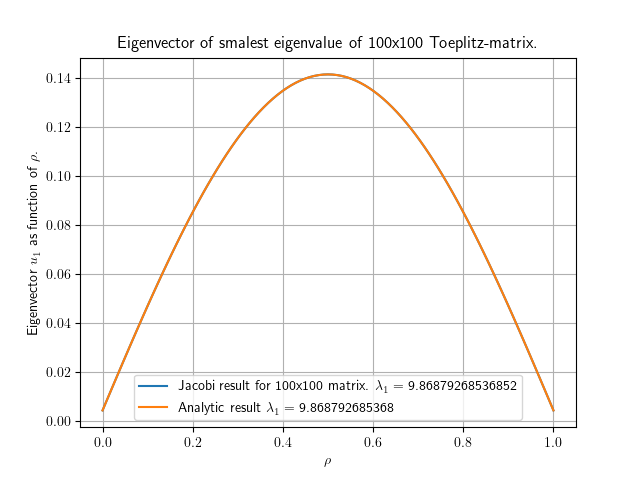
\includegraphics[width=\columnwidth]{toeplitz.png}
\caption{Plot displaying the first eigenvector calculated numerically in the buckling beam problem with $N=200$ plotted together with the analytical result. Both the analytical and numerical solution have been normalized so they are scaled similarly. The plot also shows the numerical and analytic eigenvalue belonging to this solution in the legend text.}
\end{figure}

We also measured the time spent by Jacobi's rotation algorithm and the built-in functions in the Armadillo package. This was done using a 500x500 Toeplitz matrix and 500x500 matrix from the problem of two electrons in a quantum harmonic oscillator. The results were averaged over 500 runs, and are shown in \hyperref[table:IV:a:1]{Table I}.

\begin{table}[h!] \label{table:IV:a:1}
\caption{Table showing the time spent by Jacobi's rotation algorithm and the built-in Armadillo function for finding the eigenvalues of a 500x500 Toeplitz matrix and a 500x500 matrix from the problem of two electrons in a quantum harmonic oscillator (referred to as two-electron in the table). The table shows mean time and standard deviation in seconds after 500 runs.}
\begin{tabular}{|c|c|c|}
\hline
 & Toeplitz & Two-electron \\
\hline
Jacobi & $0.0259 s \pm 0.0007$ s & $0.3672 \pm 0.0076$ s \\
Armadillo & $0.1054 \pm 0.0015$ s & $0.0910 \pm 0.0020$ s \\
\hline
\end{tabular}
\end{table}




\subsection{Quantum harmonic oscillator with one electron} \label{sec:IV:b}

We calculated the smallest four eigenvalues both numerically and analytically. They are listed in \hyperref[table:IV:b:1]{Table II} along with the relative error between them. The parameters used in this run were $N=400$ and $\rho_\text{max} = 25$. Several runs were performed keeping $N/\rho_\text{max}$ constant and the relative errors and measured values stayed almost the same.

\begin{table}[h!] \label{table:IV:b:1}
\caption{Table containing numerical and analytical eigenvalues, and the relative error between them for the single electron in a harmonic oscillator potential. The parameters used were $N=400$ and $\rho_\text{max} = 25$.}
\begin{tabular}{|c|c|c|}
\hline
Analytical & Numerical & Relative error \\
\hline
    3     &      2.999   &    $4.071 \times 10^{-4}$ \\
\hline
    7     &      6.994   &    $8.727 \times 10^{-4}$ \\
\hline
   11     &     10.985   &    $1.356 \times 10^{-3}$ \\
\hline
   15     &     14.972   &    $1.843 \times 10^{-3}$ \\
\hline
\end{tabular}
\end{table}


\subsection{Quantum harmonic oscillator with two electrons}\label{sec:IV:c}

We calculated the smallest eigenvalue for four different values of $\omega_r$ with $N=400$ and $\rho_\text{max} = 115.625$ both numerically and analytically. The eigenvalues and the relative error between them can be found in \hyperref[table:IV:c:1]{Table III}.

\begin{table}[h!] \label{table:IV:c:1}
\caption{Table containing the numerical and analytical first eigenvalue (lowest energy), and the relative error between them for the problem with two electrons in a harmonic oscillator potential. The parameters used were $N=400$ and $\rho_\text{max} = 115.625$.}
\begin{tabular}{|c|c|c|c|}
\hline
$\omega_r$ & Analytical & Numerical & Relative error \\
\hline
0.01 &    0.105    &      0.106  &    $6.966 \times 10^{-3}$ \\
\hline
0.5 &    2.057     &      2.189   &    $6.434 \times 10^{-2}$ \\
\hline
1 &   3.622     &     3.898   &    $7.623 \times 10^{-2}$ \\
\hline
5 &   14.186     &     14.118   &    $4.817 \times 10^{-3}$ \\
\hline
\end{tabular}
\end{table}

\newpage

\section{Discussion} \label{sec:V}

\subsection{Buckling beam and benchmark with Toeplitz matrix} \label{sec:V:a}

We can see in \hyperref[fig:IV:a:1]{Figure 1} that the numerically calculated eigenvector corresponds well with the analytically computed one. The numerical and analytical eigenvalues are also equal to several digits precision (more than what is shown), which together with the similar eigenvectors bode well for the accuracy of the algorithm. There are two significant sources of errors here. One is from the approximation of the second derivative, and the other is from the FLOPs performed. It is worth noting here though that the error caused by the second order derivative is not taken into account here as the analytical eigenvalues and eigenvectors used are the solutions of the eigenvalue problem with the Toeplitz matrix, and not the wave equation in general. The small error here thus shows that the error generated by the algorithm itself is not significant, but says nothing about the error from approximating the second order derivative.

Now it is important to put this back into a physical context. The eigenvectors found here correspond to stable solutions to the wave equation. In theory there is an infinite amount of these solutions, but when searching numerically the amount of solutions is limited by the dimensionality of the matrix. Just as in the case with eigenvectors the solutions can always be multiplied with a constant and still remain a valid solution. This means that normalizing the eigenvectors in \hyperref[fig:IV:a:1]{Figure 1} also makes sense in the context of the solutions to the wave equation.

From the benchmark results in \hyperref[table:IV:a:1]{Table I.}, it becomes clear that our implementation of Jacobi's rotation algorithm (\hyperref[sec:III:a]{section III A.}) finishes faster than Armadillo's eig\_sym function for the Toeplitz matrix. The Armadillo eig\_sym solver uses the divide and conquer method \citep{Armadillo} for solving the eigenpairs of symmetric matrices. The estimated maximum FLOPs needed for convergence, for a given \(N\times N\)-matrix, is \(\frac{8}{3}N^{3}\) with eigenvectors, or \(\frac{4}{3}N^{3}\) when solving for eigenvalues only \citep{Cuppen}. This is less than the estimate of between \(36N^{3}\) and \(60N^{3}\) as the maximum number of FLOPs for our implementation of Jacobi's rotation algorithm.

The Jacobi solver and the eig\_sym solver seem to converge in fewer than the maximum needed number of iterations. Our Jacobi solver is likely faster than the eig\_sym solver when solving the Toeplitz matrix, because the matrix requires few iterations to reach our set tolerance of \(\num{1e-08}\) for the maximum non-diagonal element. Armadillo's eig\_sym function probably uses a stricter tolerance, which would explain why it may spend more time in this simple case. The results in \hyperref[table:IV:a:1]{Table I.} for the two-electron matrix are as expected, with the eig\_sym solver being significantly faster than our Jacobi solver. The two-electron matrix likely requires more iterations to reach our set tolerance of \(\num{1e-08}\) for the maximum non-diagonal element and, by extension, requires closer to the maximum number of FLOPs. With more iterations needed it is also more likely that the increased efficiency of Armadillo's eig\_sym function comes to light more, which is the case here.


\subsection{Quantum harmonic oscillator} \label{sec:V:b}

\subsubsection{One electron} \label{sec:V:b:i}

We calculated the four lowest eigenvalues of the system using Jacobi's rotation algorithm, and compared them with the analytical values as seen in \hyperref[table:IV:b:1]{Table II}. In general we see that the values found numerically correspond to the analytical values. At least four the smallest four eigenvalues however, we can clearly see the relative error increasing for the larger eigenvalues. There are three significant sources of errors this time around. The analytical eigenvalues are found by solving the equation directly, which means that there is an error from approximating the second order derivative. We also have an error from the FLOPs performed and from the loss of numerical precision in the diagonal elements of the matrix as discussed in \hyperref[sec:III:b]{section III.B}. The error from the second order derivative and from the FLOPs should (logically at least) cause steady relative errors for all eigenvalues. This makes it likely that the increasing relative errors for larger eigenvalues are related to the loss of numerical precision in the diagonal elements.

We also performed several runs of this keeping $N/\rho_\text{max} = 16$ constant. The relative error and calculated eigenvalues stayed pretty much the same for all these runs, unless we picked very small values for $\rho_\text{max}$ and $N$. Very large values of $N$ is not possible to due to computational limitations but they should in theory cause similar problems to small values being chosen. As the numerically calculated eigenvalues stayed pretty much the same we conclude that there is little reason to believe the error from the FLOPs are a large contribution to the total error. The error resulting from approximating the second order derivative should be the same as long as the step length $h$ is constant, which it is in this case as $h = \rho_\text{max}/N$. This specific value was chosen because they seemed to produce results accurate to the fourth digit for the first eigenvalue which was what we sought initially.

The eigenvalues here are proportional to the allowed energy values of the system with $l=0$ by $\lambda_n = \frac{2}{\hbar \omega} E_n$, where $E_{n+1} > E_n$ for all positive integers $n$. In theory, as long as we assume the harmonic oscillator potential to be infinitely deep we have an infinite amount of allowed energies as $n$ can go to infinity. When calculating numerically, similarly to the buckling beam problem, the amount of solutions we can find are limited by the dimensionality of the matrix. It is worth noting here that generally speaking when using a harmonic oscillator potential in quantum mechanics, this is only a local approximation of a potential. Thus it is often common to define a limit to how large the energy can get before the electron escapes the potential well. This is not done in this case, and that is why there is an infinite amount of allowed energies. As the increase in the energy is linear to the increase of the energy level $n$ the relative distance between neighbouring energy levels gets smaller as $n$ gets larger and in the classical limit we get a (at least approximately) continuous spectrum of allowed energies. It is not feasible to reach this point when solving this problem numerically however as this would mean having very large matrices which is just not possible without very large amounts of memory.


\subsubsection{Two electrons} \label{sec:V:b:ii}

We calculated the eigenvalues for the quantum harmonic oscillator system with two electrons for different choices of $\omega_r$ and recorded the smallest ones in \hyperref[table:IV:c:1]{Table III} along with the analytical values and the relative error between these. These eigenvalues are dimensionless and proportional to the relative energy between the electrons in the ground state. As in the previous problems there is generally an infinite set of solutions as long as we assume the potential well of the harmonic oscillator to be infinitely deep, but the amount of solutions we can find numerically is limited by the dimensionality of the matrix used.

In this case $N/\rho_\text{max} \approx 3.46$ seemed to provide the best results, even though the relative error in this case is quite large compared to the previous two problems. Important things to note here compared to the problem with one electron, in terms of possible sources of errors, are that the step length is significantly larger, and that the error in the diagonal elements of the matrix also is larger due to the extra term (see \hyperref[sec:III:b]{section III.B.} and \hyperref[sec:II:e]{section II.E.}). The larger step length causes the error in the approximation of the second order derivative to be much worse, but it is unlikely that this is the only cause of the increase in relative error. Notably the most similar case to the previous problem is when $\omega_r = 1$, and here the relative error is significantly larger.

We would also expect the relative error for different $\omega_r$ to be better for different choices of $N/\rho_\text{max}$, but choosing a single value better highlights the problems encountered when trying to solve this problem numerically. As expected we can clearly see that the relative error varies for different $\omega_r$, but we can also see, interestingly enough, that it seems to reach a peak at some point between $\omega_r = 0.5$ and 1. If we did the calculations for even more $\omega_r$ this trend would be easier to verify, but this is something we leave for further research. If this is in fact a peak of the relative error, and not just some artifact of us not having enough data, this could indicate that there is a point where the differences between the terms in the diagonal elements of the matrix (see \hyperref[sec:III:b]{Section III.B.}) causes the error to reach a maximum for a given choice of $N/\rho_\text{max}$.

With these things taken into consideration it seems very difficult to solve this kind of system numerically, as we need to take a guess at several parameters. The error would also vary throughout even a single solution, and quantifying the behaviour of the error would then be necessary in order to obtain more accurate results. With the amount of data we have here it is not possible to quantify the error in such a way, and a more thorough study of this system in particular would be necessary. As the main purpose of this report is to evaluate our implementation of Jacobi's rotation algorithm, we leave any further quantifying of the behaviour of the relative error to further research. It is also difficult in this case to say much about the error caused by Jacobi's rotation algorithm, especially as the other sources of errors are so significant. Comparing against other methods is also complicated as we would need to know the error caused by those methods in order to determine the error caused by our implementation of Jacobi's rotation algorithm, which again would require more knowledge about how the error behaves in this specific system. \newline \newline

\newpage
\section{Conclusion} \label{sec:VI}
In this report we have presented an implementation of Jacobi's rotational algorithm for finding the eigenpairs of symmetric matrices. We used our implementation to obtain approximate solutions for the eigenpairs of the \(1\)st vibrational mode of a buckling beam, the four lowest energies of a single electron in a quantum harmonic oscillator potential, as well as the ground-state energies of two electrons in a quantum harmonic oscillator potential with different values of the scaled frequency \(\omega_{r}\).

By solving the buckling beam problem, our implementation gave results that matched the analytic solution (see \hyperref[fig:IV:a:1]{Figure 1}). Furthermore, we compared the computational speed of our implementation to the eigenpair solver for symmetric matrices, eig\_sym, in the Armadillo C++ library. The benchmark comparison revealed our implementation to be faster than the eig\_sym solver (see \hyperref[table:IV:a:1]{Table I}). This might be because the maximum number of FLOPs of our implementation is between \(36N^{3}\) and \(60N^{3}\) for an \(N\times N\)-matrix, while the method employed by eig\_sym requires a maximum of \(\frac{8}{3}N^{3}\) FLOPs to complete \citep{Cuppen}. Moreover, the benchmark was performed on a \(500\times 500\)-Toeplitz matrix. This is a rather simple matrix, and likely does not require many iterations to reach the tolerance of \(\num{1e-08}\) set for the maximum non-diagonal element. A similar benchmark performed with the matrix from the two-electron problem gave the expected result of eig\_sym being faster than the Jacobi solver.

For the two quantum harmonic oscillator problems we saw an expected increase in the relative error of our results. We conclude that these errors mostly arise from loss of numerical precision in generating the matrices we find the eigenvalues of, and from approximation of the second order derivative which are both unrelated to the algorithm used to find the eigenvalues. In the case of the one electron case specifically the choice of parameters that minimizes these sources of errors significance contradict eachother, creating difficulties in solving the problem numerically. This also makes it difficult to use the results here to assess the size of the relative error caused by the algorithm alone. In the case of two electrons we know even less about the behaviour of the relative error from setting up the problem. It would be necessary to quantify the behaviour of the relative error from setting up the matrix further in order to use this problem to evaluate our implementation, and as this is a project large enough to warrant a separate study we leave this for further research.

\onecolumngrid
\bibliography{kilder.bib}{}
\newpage
\twocolumngrid

\appendix
\section{Source code} \label{A}
All code for this report was written in C++ and Python 3.8, and the complete set of files can be found at
\url{https://github.com/eivinsto/FYS3150_Project2.git}.

\cprotect\subsection{\verb+project.py+} \label{A.1}
Main script for running project, plotting and data analysis.

\url{https://github.com/eivinsto/FYS3150_Project2/blob/master/project.py}

\cprotect\subsection{\verb+main.cpp+} \label{A.2}
Main cpp file for running algorithms.

\url{https://github.com/eivinsto/FYS3150_Project2/blob/master/src/main.cpp}

\cprotect\subsection{\verb+functions.cpp+} \label{A.3}
File contaning functions for creating the matrices used in the project, and calculating analytical eigenvalues and eigenvectors.

\url{https://github.com/eivinsto/FYS3150_Project2/blob/master/src/functions.cpp}

\cprotect\subsection{\verb+jacobi.h+} \label{A.4}
File containing the decleration of a jacobi\_solver class, and jacobi\_functions class.

\url{https://github.com/eivinsto/FYS3150_Project2/blob/master/src/jacobi_solver.h}

\cprotect\subsection{\verb+jacobi.cpp+} \label{A.5}
File containing the class-methods for the jacobi classes. Including the implementation of Jacobi's rotational algorithm.

\url{https://github.com/eivinsto/FYS3150_Project2/blob/master/src/jacobi_solver.cpp}

\cprotect\subsection{\verb+test_main.cpp+} \label{A.6}
File running unit-tests using CATCH2 framework.

\url{https://github.com/FunkMarvel/FYS3150_Project_1/blob/master/src/special_main.cpp}

\cprotect\subsection{\verb+test_functions.cpp+} \label{A.7}
File containing the unit-tests for the jacobi classes.

\url{https://github.com/eivinsto/FYS3150_Project2/blob/master/src/test_functions.cpp}

\newpage
\section{Selected results} \label{B}
Here is a folder of selected results from running our code.

\url{https://github.com/eivinsto/FYS3150_Project2/tree/master/data}

Plot can be found in doc.

\url{https://github.com/eivinsto/FYS3150_Project2/blob/master/doc/toeplitz.png}

\newpage
\section{System specifications} \label{C}
All results included in this report were achieved by running the implementation on the following system:
\begin{itemize}
	\item CPU: AMD Ryzen \(9\) \(3900\)X
	\item RAM: \(2\times\SI{8}{\giga\byte}\) Corsair Vengeance LPX DDR\(4\) \(\SI{3200}{\mega\hertz}\)
\end{itemize}
\end{document}
